% !TeX document-id = {c68f4be8-c497-43e0-82df-e9ebfbea9577}
% !TeX TXS-program:pdflatex = pdflatex -synctex=1 -interaction=nonstopmode --shell-escape %.tex
% новая команда \RNumb для вывода римских цифр
\documentclass[a4paper,12pt]{article}
\usepackage{amssymb}
\usepackage{amsmath}
\usepackage{amsthm} 
\usepackage{caption}
\usepackage{misccorr}
\usepackage[noadjust]{cite}
\usepackage{cmap} 
\usepackage[utf8]{inputenc}
\usepackage[T2A]{fontenc}
\usepackage[english, russian]{babel}
\usepackage{graphics}
\usepackage{graphicx}
\usepackage{textcomp}
\usepackage{verbatim}
\usepackage{makeidx}
\usepackage{geometry}
\usepackage{float}
\usepackage{bm}
\usepackage{esint}
\usepackage{mathtools}
\usepackage{graphicx}
\usepackage{listings}
\usepackage{courier}
\usepackage{multirow}
\usepackage{graphicx}
\usepackage[table]{xcolor}
\usepackage{color}
\usepackage[most]{tcolorbox} 
\usepackage{diagbox}

\lstset{basicstyle=\fontsize{10}{10}\selectfont,breaklines=true}

\newcommand{\specchapter}[1]{\chapter*{#1}\addcontentsline{toc}{chapter}{#1}}
\newcommand{\specsection}[1]{\section*{#1}\addcontentsline{toc}{section}{#1}}
\newcommand{\specsubsection}[1]{\subsection*{#1}\addcontentsline{toc}{subsection}{#1}}
\newcommand{\RNumb}[1]{\uppercase\expandafter{\romannumeral #1\relax}}
\newcommand{\jj}{\righthyphenmin=20 \justifying}


% геометрия
\geometry{pdftex, left = 2cm, right = 2cm, top = 2.5cm, bottom = 2.5cm}

\setcounter{tocdepth}{4} % фикс переноса 
\righthyphenmin = 2
\tolerance = 2048

\begin{document}
	\thispagestyle{empty}
	
	\noindent \begin{minipage}{0.15\textwidth}
		
\includegraphics[width=\linewidth]{b_logo}
	\end{minipage}
	\noindent\begin{minipage}{0.9\textwidth}\centering
		\textbf{Министерство науки и высшего образования Российской Федерации}\\
		\textbf{Федеральное государственное бюджетное образовательное учреждение высшего образования}\\
		\textbf{«Московский государственный технический университет имени Н.Э.~Баумана}\\
		\textbf{(национальный исследовательский университет)»}\\
		\textbf{(МГТУ им. Н.Э.~Баумана)}
	\end{minipage}
	
	\noindent\rule{18cm}{3pt}
	\newline\newline
	\noindent ФАКУЛЬТЕТ $\underline{\text{«Информатика и системы управления»}}$ \newline\newline
	\noindent КАФЕДРА $\underline{\text{«Компьютерные системы и сети»}}$\newline\newline
	\noindent НАПРАВЛЕНИЕ ПОДГОТОВКИ $\underline{\text{«09.03.04 Программная инженерия»}}$\newline\newline\newline\newline\newline
	
	
	\begin{center}
		\noindent\begin{minipage}{1.3\textwidth}\centering
			\Large\textbf{  Рубежный контроль по  }\newline
			\Large\textbf{ дисциплине <<Архитектура ЭВМ>>}\newline\newline\newline
			\textbf{Классификация и основные характеристики ПЗУ.}\newline
			\textbf{ ~~~~~~   Элементная база ПЗУ. }\newline\newline\newline\newline
		\end{minipage}
	\end{center}
	
	\begin{center}
		\begin{tabular}{ccccc}
			Студент: & $\underline{\text{ИУ7-53Б}}$ & $\underline{\text{~~~~~~~~~~~}}$ & $\underline{\text{23.12.2020}}$ & $\underline{\text{А. В. Романов}}$ \\
			& \footnotesize группа & \footnotesize подпись & \footnotesize дата  & \footnotesize (И. О. Фамилия) \\
			&  &  &  & \\
			Преподаватель: & \textbf{} & $\underline{\text{~~~~~~~~~~~}}$ & $\underline{\text{~~~~~~~~~~~~}}$ & $\underline{\text{А. Ю. Попов}}$ \\
			&  & \footnotesize подпись & \footnotesize дата  & \footnotesize (И. О. Фамилия) \\
		\end{tabular}
	\end{center}
	
	
	\begin{center}
		\vfill
		Москва~---~\the\year
		~г.
	\end{center}
	\clearpage
	
	
	\begin{center}
		\noindent 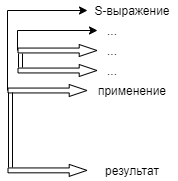
\includegraphics[scale=0.5]{1.png}\newline
	\end{center}

	Постоянные запоминающие устройства (память типа Read Only Memory) -- хранят информацию которая не меняется (либо меняется редко, в специальном режиме). В ПЗУ хранится предварительно занесенная информация. 
	Требования к ПЗУ: энергонезависимость. 
	
	Классификация ПЗУ: 
	
	\begin{itemize}
		\item Масочные ПЗУ -- самые быстродействующие ЗУ. Туда нельзя записать, можно только прочитать. Изменить информацию можно только в специальном режиме, не доступном пользователю. Запоминающие элементы могут быть реализованы \textbf{на диодах} или на \textbf{МОП транзисторах.}
		\item Программируемые ПЗУ. Такие ПЗУ, которые можно перепрограммировать в лабораторных условиях (т.е. не на заводе). Варианты реализаций: ППЗУ \textbf{с плавкими перемычками} или \textbf{с пережигаемым p-n переходом}.
		\item Репрограммируемые ПЗУ. в такую память можно записать что-либо ограниченное количество раз. Существует реализация РПЗУ \textbf{с записью электрическими сигналами и стиранием ультрафиолетовым излучением}. Ультрафиолет плохо влияет на материалы и РПЗУ деградирует. Так же существует реализация \textbf{с транзисторами <<плавающим>> забором.}
	\end{itemize}

	ПЗУ работают только в режимах хранения либо считывания. Элементная база ПЗУ состоит из:
	\begin{itemize}
		\item Накопитель -- матрица элементов памяти.
		\item Элемент памяти.
		\item Программируемая перемычка (в виде полупроводниковых диодов или транзисторов, включенные между строками и столбцами матрицы). Наличие перемычки можно использовать как логическую единицу, а отсутствие -- нулю. Таким образом реализуется требование энергонезависимость.
	\end{itemize}

	Микросхемы ПЗУ имеют словарную организацию, информация считывается в форме слова. Совокупность элементов памяти в матрице накопителя, хранящих слово -- ячейка, каждая такая ячейка имеет свой адрес.

\end{document}